\documentclass{article}

\usepackage{hyperref}
\hypersetup{
    colorlinks=true,
    linkcolor=blue,
    filecolor=magenta,      
    urlcolor=cyan,
}

% for including notebooks
\usepackage{pdfpages}
\usepackage{fancyhdr}
\usepackage{extramarks}
\usepackage{amsmath}
\usepackage{amsthm}
\usepackage{amsfonts}
\usepackage{tikz}
\usepackage{float}
\usepackage[plain]{algorithm}
\usepackage{algpseudocode}
\usepackage{caption}
\usepackage{subcaption}
\usepackage[toc,page]{appendix}
\usepackage{siunitx}
\usepackage{footnote}

\usepackage{listings}
\usepackage{color}
\definecolor{mygreen}{RGB}{28,172,0} 
\definecolor{mylilas}{RGB}{170,55,241}

\lstset{
    basicstyle=\scriptsize\sffamily\color{black},
    frame=single,
    numbers=left,
    showspaces=false,
    showstringspaces=false,
    tabsize=1
}
\lstset{language=Matlab,%
    %basicstyle=\color{red},
    breaklines=true,%
    morekeywords={matlab2tikz},
    keywordstyle=\color{blue},%
    morekeywords=[2]{1}, keywordstyle=[2]{\color{black}},
    identifierstyle=\color{black},%
    stringstyle=\color{mylilas},
    commentstyle=\color{mygreen},%
    showstringspaces=false,%without this there will be a symbol in the places where there is a space
    numbers=left,%
    numberstyle={\tiny \color{black}},% size of the numbers
    numbersep=9pt, % this defines how far the numbers are from the text
    emph=[1]{for,end,break},emphstyle=[1]\color{red}, %some words to emphasise
    %emph=[2]{word1,word2}, emphstyle=[2]{style},    
}

\topmargin=-0.45in
\evensidemargin=0in
\oddsidemargin=0in
\textwidth=6.5in
\textheight=9.0in
\headsep=0.25in


\linespread{1.1}

\pagestyle{fancy}
\fancyhf{}
\lhead{\hmwkAuthorName}
\chead{\hmwkClass: \hmwkTitle}
\rhead{\leftmark}
\lfoot{\lastxmark}
\cfoot{\thepage}

\renewcommand\headrulewidth{0.4pt}
\renewcommand\footrulewidth{0.4pt}

\setlength\parindent{0pt}

\newcommand{\hmwkTitle}{Assignment \ 3}
\newcommand{\hmwkDueDate}{April 1, 2020}
\newcommand{\hmwkClass}{Control Theory}
\newcommand{\hmwkClassInstructor}{Mike Ivanov}
\newcommand{\hmwkAuthorName}{\textbf{Artem Bakhanov (B18-03)}}

%
% Title Page
%

\title{
    \vspace{2in}
    \textmd{\textbf{\hmwkClass:\ \hmwkTitle}}\\
    \normalsize\vspace{0.1in}\small{Due\ on\ \hmwkDueDate\ at 11:59pm}\\
    \vspace{0.1in}\large{\textit{\hmwkClassInstructor\ }}
    \vspace{3in}
}

\author{\hmwkAuthorName}
\date{}

\begin{document}

\maketitle

\pagebreak

\tableofcontents

\pagebreak

\section{Introduction}
    I created a GitHub repository \href{https://github.com/artembakhanov/ControlTheoryHomework}{here}.
    All the problems are solved by me, Artem Bakhanov, a student of Innopolis University. My variant is \textbf{g}.
\section{Python}
For the first task I used Python to calculate everything. You can find the code in Appendix 1 in the end of the document.
\subsection{A}
In this subtask I tested 2 trajectories: $\overset{*}{x} = 1$ and $\overset{*}{x} = 4$. Zero-conditions are $x(0) = .28789452$ and $x'(0) = .72404173$
\begin{figure}[ht]
        \centering
        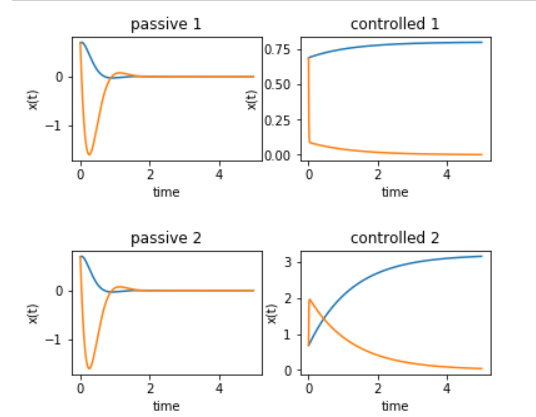
\includegraphics[width=0.7\textwidth]{images/1}
        \caption{Two trajectories}
        \label{fig:plot1a}
\end{figure}
\subsection{B}
For this part I used a process described on \href{https://en.wikipedia.org/wiki/PID_controller#Manual_tuning}{Wikipedia}. I got parameters $k_p = 2000$ and $k_d = 300$. Trajectories are the same.
I used step with amplitude 1 and starting time 0.5. On the plots below you can see that the PD controller works but not perfectly. I-component is missing.
\begin{figure}[H]
        \centering
        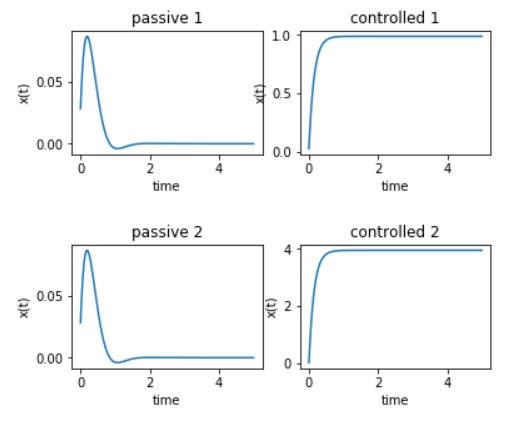
\includegraphics[width=0.7\textwidth]{images/2}
        \caption{Tuned PD}
        \label{fig:plot1b_1}
\end{figure}
\begin{figure}[H]
        \centering
        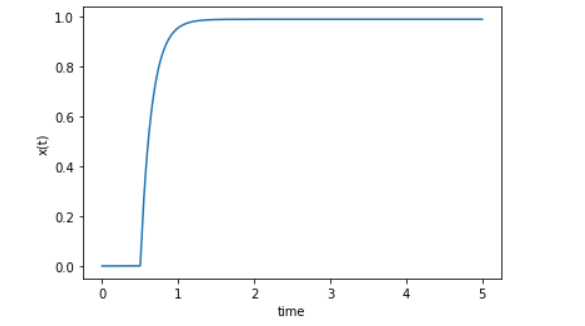
\includegraphics[width=0.7\textwidth]{images/3}
        \caption{Step response. $t_0 = 0.5$}
        \label{fig:plot1b_2}
\end{figure}
\subsection{C}
For this part I used built-in Matlab function \texttt{isstable}. The function proved that the controlled oscillator dynamics is stable for $k_p = 2000$ and $k_d = 300$. You can find the code below. 
\lstinputlisting[caption=Stability proof, label={lst:listing1}, language=Matlab, captionpos=b, float=ht]{code/task2c.m}
\subsection{D}
The solution is pretty the same but the parameters are different. You can look at my code in the Appendix 1. I did not get how we can do something with the system where we do not know the B matrix, so I assumed that $B = \begin{bmatrix}
        0\\ 
        1
    \end{bmatrix}$. The problem is that I did not understand how to get the parameters, since it is now a numbers but matrices.
\subsection{E}
The PID controller is very similar to what was done in the task B. 
I found PID parameters by hand and got: 150, 130, and 25 for $k_p$, $k_i$, and $k_d$ respectively.
\begin{figure}[ht]
   	 \centering
     \begin{subfigure}[b]{0.45\textwidth}
         \centering
         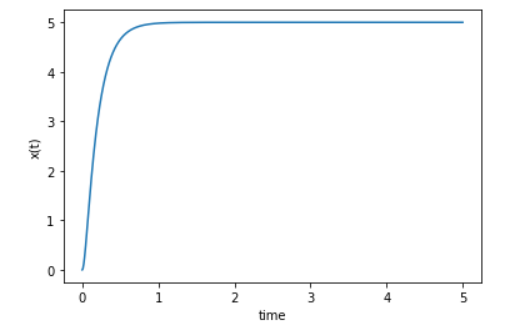
\includegraphics[width=\textwidth]{images/8.png}
         \caption{Desired x: 5}
         \label{fig:test1}
     \end{subfigure}
     \hfill
     \begin{subfigure}[b]{0.45\textwidth}
         \centering
         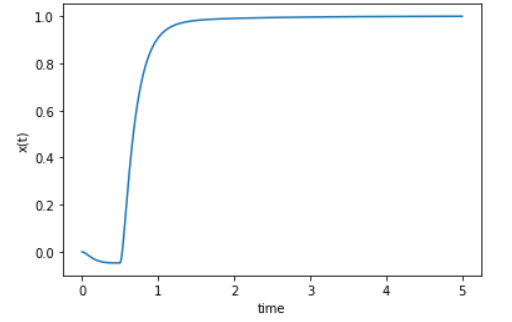
\includegraphics[width=\textwidth]{images/9.png}
         \caption{Step response with amplitude 1 and time 0.5}
         \label{fig:test2}
     \end{subfigure}
     \caption{Examples of tests.}
\end{figure}
\section{PID Tuner}
In this section I used Simulink for analyzing the system and PIDTuner to tune the PID controller in the system. The system looks like:
\begin{figure}[H]
        \centering
        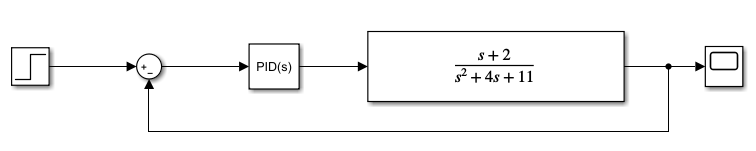
\includegraphics[width=0.7\textwidth]{images/7}
        \caption{The system}
        \label{fig:plot3_1}
\end{figure}
The parameters that PIDTuner gave me: $k_p = 10.826321698108$, $k_i = 63.4181190369928$, and $k_d = -0.0076494311467772$. The step input (amplitude = 5) was used and the trajectory of the system is on the picture below.
\begin{figure}[H]
        \centering
        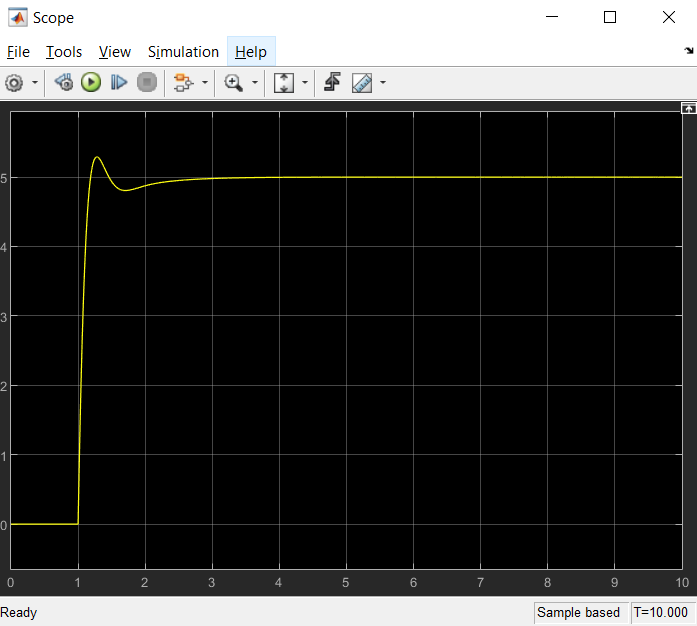
\includegraphics[width=0.5\textwidth]{images/6}
        \caption{The system trajectory}
        \label{fig:plot3_2}
\end{figure}
\begin{appendices}
\section{Python Code}
\label{appendix:code}
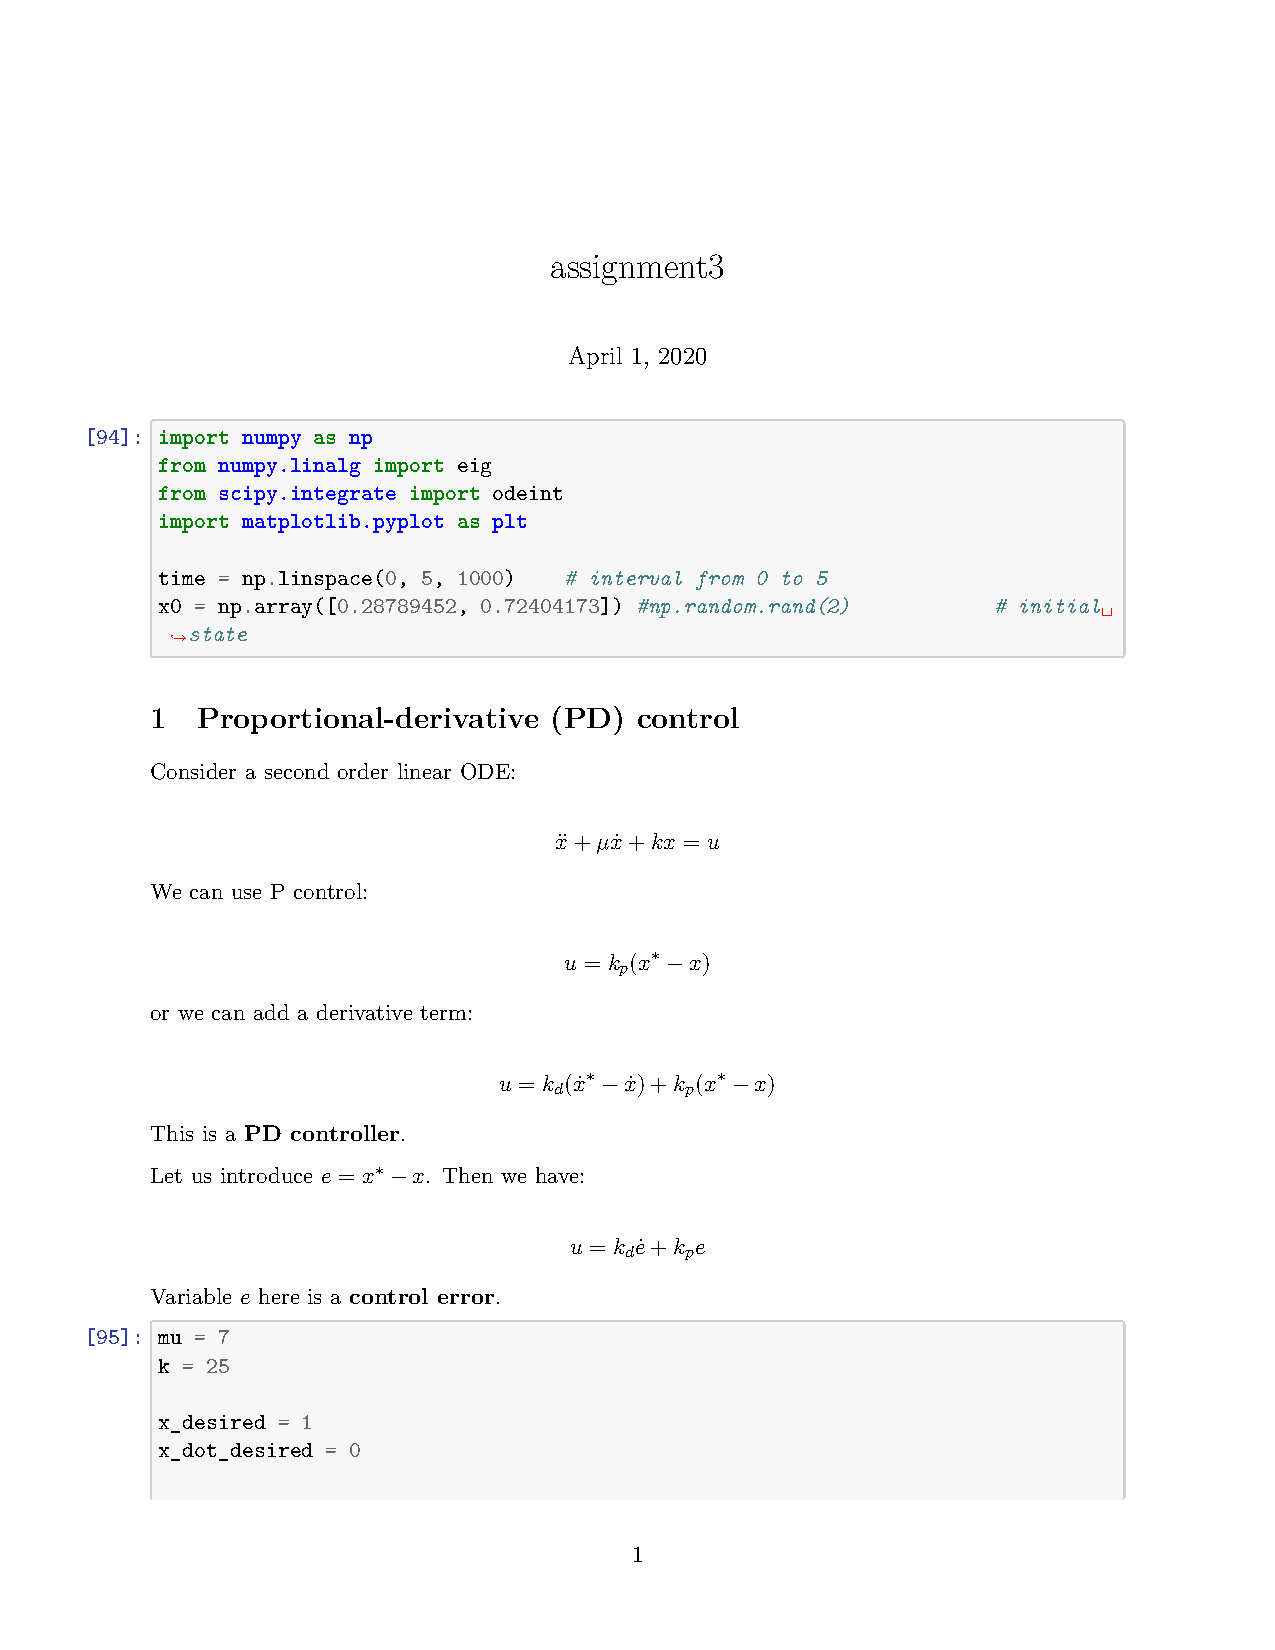
\includegraphics[page=1,width=\textwidth]{code/python.pdf}
    \includepdf[pages=2-,pagecommand={},width=\textwidth]{code/python.pdf}
\end{appendices}
\end{document}

